\input{preambule_article}
\usepackage{adjustbox}

%TODO
% 1) Add errors for correlation coefficients
% 2) 
\begin{document}
\begin{center}
    
    \normalsize{Федеральное государственное автономное образовательное учреждение высшего образования}
    
    \textbf{НАЦИОНАЛЬНЫЙ ИССЛЕДОВАТЕЛЬСКИЙ УНИВЕРСИТЕТ \\ <<МОСКОВСКИЙ ФИЗИКО-ТЕХНИЧЕСКИЙ ИНСТИТУТ>>}
    \vspace{13ex}
    
    \textbf{Отчет по лабораторной работе 5.4 <<Компьютерная сцинитилляционная $\gamma$ - спектрометрия >> }
    
    \vspace{40ex}
\end{center}
\begin{flushright}
    \normalsize{Выполнил: Сидельников Станислав Игоревич \\ студент Б01-908\\}
\end{flushright}
    
\vfill
    
\begin{center}
Долгопрудный, 2021
\end{center}

\thispagestyle{empty} % выключаем отображение номера для этой страницы

\newpage
	\section{Аннотация}
	
	\textbf{Цель работы:} исследование при помощи спектрометрии
						  эффектов рассеяния $\gamma$-квантов на различных типах веществ. 
	
	
	\textbf{В работе используются:}
	
	\begin{itemize}
		
		\item сцинтиллятор
		\item ФЭУ
		\item предусилитель импульсов
		\item высоковольтный блок питания для ФЭУ
		\item АЦП
		\item компьютер
		
	\end{itemize}
	
	\section{Теоретические сведения}
	
	\textbf{Фотоэффект} - это процесс взаимодействия гамма-кванта с электроном, связанным с атомом, при котором электрону передается вся энергия гамма-кванта. При этом электрону сообщается кинетическая энергия $T_e=E_\gamma-I_i$, где $E_\gamma$ -- энергия гамма-кванта, $I_i$ -- потенциал ионизации $i$-той оболочки атома. Фотоэффект особенно существенен для тяжелых веществ, где он идет с заметной вероятностью даже при высоких энергиях гамма-квантов. В легких веществах фотоэффект становится заметен лишь при относительно небольших энергиях гамма-квантов.  \par
	\textbf{Эффект Комптона} - это упругое рассеяние фотона на свободном электроне, сопровождающееся изменением длины волны фотона. Максимальная энергия образующихся комптоновских электронов соответствует рассеянию гамма-квантов на $180^\circ$ и равна
	\begin{equation}
		E_{\max}=\frac{h\omega}{1+\frac{mc^2}{2h\omega}}.
	\end{equation}
	\textbf{Процесс образования электрон-позитронных пар.}
	При достаточно высокой энергии гамма-кванта наряду с фотоэффектом и эффектом Комптона может происходить третий вид взаимодействия гамма-квантов с веществом -- образование электрон-позитронных пар. Процесс образования пар не может происходить в пустоте, так как в этом случае не выполняются законы сохранения энергии и импульса. В присутствии ядра или электрона процесс образования пары гамма-квантов возможен, так как можно распределить энергию и импульс гамма-кванта между тремя частицами без противоречия с законами сохранения. При этом если процесс образования пары идет в кулоновском поле ядра или протона, то энергия образующегося ядра отдачи оказывается весьма малой, так что пороговая энергия гамма-кванта $E_0$, необходимая для образования пары, практически совпадает с удвоенной энергией покоя электрона $E_0\cong 2mc^2=1.022$ МэВ.\par
	Появившийся в результате процесса образования пар электрон свою энергию на ионизацию среды. Таким образом, вся энергия электрона остается в детекторе. Позитрон будет двигаться до тех пор, пока практически не остановится, а затем аннигилирует с электроном среды, в результате чего появятся два гамма-кванта. Т.е., кинетическая энергия позитрона также останется в детекторе. Далее возможны три варианта развития событий:
	\begin{enumerate}
		\item оба родившихся гамма-кванта не вылетают из детектора, и тогда вся энергия первичного гамма-кванта останется в детекторе, а в спектре появится пик с $E=E_{\gamma}$;
		\item один из родившихся гамма-квантов покидает детектор, и в спектре появляется пик, соответствующий энергии $E=E_{\gamma}-E_0$, где $E_0=mc^2=511$ кэВ;
		\item оба родившихся гамма-кванта покидают детектор, и в спектре появляется пик, соотвествующий энергии $E=E_{\gamma}-2E_0$, где $2E_0=2mc^2=1022$ кэВ.
	\end{enumerate}
	Таким образом, любой спектр, получаемый с помощью гамма-спектрометра, описывается несколькими компонентами, каждая из которых связана с определенным физическим процессом. Как описано выше, основными физическими процессами взаимодействия гамма-квантов с веществом является фотоэффект, эффект Комптона и образование электрон-позитронных пар, и каждый из них вносит свой вклад в образование спектра. Помимо этих процессов, добавляется \textit{экспонента}, связанная с наличием фона, \textit{пик характеристического излучения}, возникающий при взаимодействии гамма-квантов с окружающим веществом, а также \textit{пик обратного рассеяния}, образующийся при энергии квантов $E_{\gamma}\gg mc^2/2$ в результате рассеяния гамма-квантов на большие углы на материалах  конструктивных элементов детектора и защиты. Положение пика обратного рассеяния определяется по формуле:
	\begin{equation}
		E_{\text{обр}}=\frac{E}{1+2E/mc^2},
		\label{eq:Ereverse}
	\end{equation}
	где $E$ -- энергия фотопика.\par
	\paragraph{Энергетическое разрешение спектрометра.} Даже при поглощении частиц с одинаковой энергией амплитуда импульса на выходе фотоприёмника сцинтилляционного детектора меняется от события к событию. Это связано:
	\begin{enumerate}
		\item со статистическим характером процессов сбора фотонов на фотоприёмнике и последующего усиления,
		\item с различной вероятностью доставки фотона к фотоприемнику из разных точек сцинтиллятора,
		\item с разбросом высвечиваемого числа фотонов
	\end{enumerate}
	\par
	В результате в набранном спектре линия (которая для идеального детектора представляла бы дельта-функцию) оказывается размытой, её часто описывают гауссианом.\par
	Энергетическим разрешением спектрометра называется величина
	\begin{equation}
		R_i=\frac{\Delta E_i}{E_i},
	\end{equation}
	где $\Delta E_i$ -- ширина пика полного поглощения, измеренная на половине высоты, $E_i$ -- энергия регистрируемого $\gamma$-излучения. Значение $E_i$ пропорционально среднему числу фотонов $\overline{n_i}$ на выходе ФЭУ, т.е.:
	\begin{equation}
		E_i=\alpha\overline{n_i}.
		\label{eq:4}
	\end{equation}
	\par
	Полуширина пика полного поглощения $\Delta E_i$ пропорциональна среднеквадратичной флуктуации $\overline{\Delta n_i}$. Т.к. $n_i$ является дискретной случайной величиной, которая распределена по закону Пуассона, то $\overline{\Delta n_i}=\sqrt{\overline{n_i}}$ и поэтому
	\begin{equation}
		\Delta E_i=\alpha\overline{\Delta n_i}=\alpha\sqrt{\overline{n_i}}.
		\label{eq:5}
	\end{equation}
	\par
	Из (\ref{eq:4}), (\ref{eq:5}) получаем, что
	\begin{equation}
		R_i=\frac{\Delta E_i}{E_i}=\frac{\text{const}}{\sqrt{E_i}}.
		\label{eq:6}
	\end{equation}
	\par
	Поскольку энергетическое разрешение зависит от энергии, его следует указывать для конкретной энергии. Чаще всего разрешение указывают для энергии гамма-линии $^{137}\text{Cs}$ (661.7 кэВ).
	
	\section{Результаты измерений и обработка данных}
	
	\subsection{Определение зависимости между энергией гамма квантов и номерами каналов}
	
	Здесь и далее погрешность определение пиков считаем равной 10 каналам, и она определяется
	ошибкой определения номера канала при снятии на глаз пика с графика на компьютере.
	
	\[\delta_{ch} = 10\]
	
	
\begin{table}[h]
	\begin{tabular}{|l|l|l|}
		\hline
		\begin{tabular}[c]{@{}l@{}}Результаты измерения фотопиков\\ для калибровочных данных\end{tabular} &              &             \\ \hline
		& Номер канала & Энергия, эВ \\ \hline
		Фотопик Na                                                                                        & 1742         & 1275000     \\ \hline
		Анигиляционный пик Na                                                                             & 746          & 511000      \\ \hline
		Фотопик Cs                                                                                        & 942          & 661700      \\ \hline
	\end{tabular}
\end{table}

\newpage

	\begin{figure}[h]
		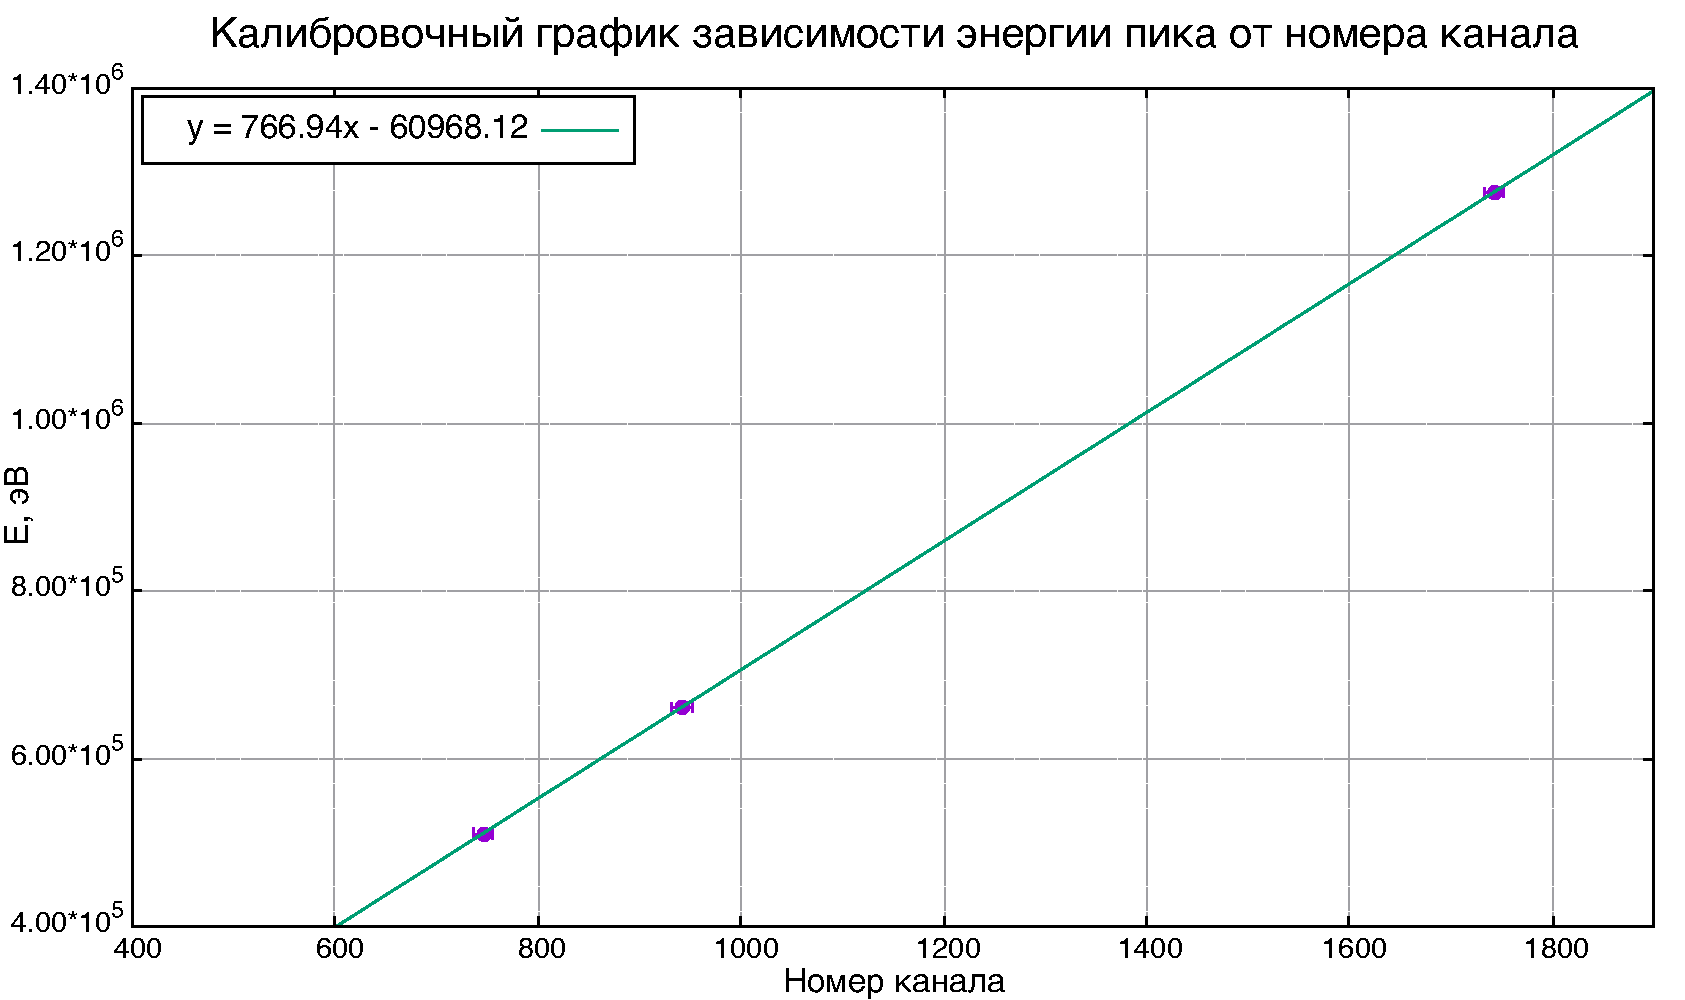
\includegraphics[width=\linewidth]{../data/correlation.pdf}
	\end{figure}
	
	Коэффиценты, вычисленные согласно калибровочному графику:
	
	\[ E = 766.94 \cdot N + 60968.12 \text{, где N - номер канала}\]
	
	\subsection{Измерения пиков, ширины пиков и разрешающей способности}
	
	
	Погрешность измерения энергии, учитывая линейную зависимость
	от погрешность измерения коэффициента перевода номера канала в энергию:

	\[ \delta_{E} = a \cdot \delta_{N} = 7669\]
	
	Погрешность измерения ширины пика:
	
	\[ \delta_{dE} = a \cdot \delta_{dN} = 7669\]
	
	Погрешность измерения энергетического разрешения:
	
	\[ \delta_{R} = 0.02 \]
	
	\newpage
	
	\begin{table}[]
		\begin{tabular}{|l|l|l|l|}
			\hline
			Элемент & N, номер канала & \begin{tabular}[c]{@{}l@{}}Погрешность измерения\\ номера канала\end{tabular} & dN, ширина\\ \hline
			Co60    & 1825            & 10                                                                            & 223             \\ \hline
			-//-    & 1607            & 10                                                                            & 183             \\ \hline
			Na      & 1742            & 10                                                                            & 168             \\ \hline
			Cs      & 942             & 10                                                                            & 147             \\ \hline
			Am      & 161             & 10                                                                            & 55              \\ \hline
			Eu      & 527             & 10                                                                            & 110             \\ \hline
			-//-    & 400             & 10                                                                            & 58              \\ \hline
			-//-    & 243             &                                                                               & 55              \\ \hline
		\end{tabular}
	\end{table}

\begin{table}[h]
	\begin{tabular}{|l|l|l|l|}
		\hline
		Элемент & \begin{tabular}[c]{@{}l@{}}Погрешность\\ ширины \end{tabular} & E, значение энергии в эВ & \begin{tabular}[c]{@{}l@{}}Погрешность измерения\\ энергии\end{tabular} \\ \hline
		Co60    & 20                                                                          & 1338697.37726            & 7669                                                                    \\ \hline
		-//-    & 20                                                                          & 1171504.45726            & 7669                                                                    \\ \hline
		Na      & 20                                                                          & 1275041.35726            & 7669                                                                    \\ \hline
		Cs      & 20                                                                          & 661489.35726             & 7669                                                                    \\ \hline
		Am      & 20                                                                          & 62509.21726              & 7669                                                                    \\ \hline
		Eu      & 20                                                                          & 343209.25726             & 7669                                                                    \\ \hline
		-//-    & 20                                                                          & 245807.87726             & 7669                                                                    \\ \hline
		-//-    & 20                                                                          & 125398.29726             & 7669                                                                    \\ \hline
	\end{tabular}
\end{table}

\begin{table}[h]
	\begin{tabular}{|l|l|l|l|l|}
		\hline
		Элемент & \begin{tabular}[c]{@{}l@{}}dE, ширина пика\\ в эВ\end{tabular} & \begin{tabular}[c]{@{}l@{}}Погрешность \\ измерения\\ ширины\\ пика, эВ\end{tabular} & \begin{tabular}[c]{@{}l@{}}Погрешность \\ энергетического\\ разрешения\end{tabular} & \begin{tabular}[c]{@{}l@{}}R, энерг.\\ разрешение\end{tabular} \\ \hline
		Co60    & 171027.62                                                      & 15334                                                                                & 0.02                                                                                & 0.127756745404293                                              \\ \hline
		-//-    & 140350.02                                                      & 15334                                                                                & 0.02                                                                                & 0.119803231759153                                              \\ \hline
		Na      & 128845.92                                                      & 15334                                                                                & 0.02                                                                                & 0.101052345687738                                              \\ \hline
		Cs      & 112740.18                                                      & 15334                                                                                & 0.02                                                                                & 0.170433853186979                                              \\ \hline
		Am      & 42181.7                                                        & 15334                                                                                & 0.02                                                                                & 0.674807681954327                                              \\ \hline
		Eu      & 84363.4                                                        & 15334                                                                                & 0.02                                                                                & 0.245807472308622                                              \\ \hline
		-//-    & 44482.52                                                       & 15334                                                                                & 0.02                                                                                & 0.180964582973674                                              \\ \hline
		-//-    & 42181.7                                                        & 15334                                                                                & 0.02                                                                                & 0.33638176053173                                               \\ \hline
	\end{tabular}
\end{table}

	\newpage

	\subsection{Исследование соответствия измеренного края комптоновского рассеяния от теоретического}
	
	
	\begin{figure}[h]
	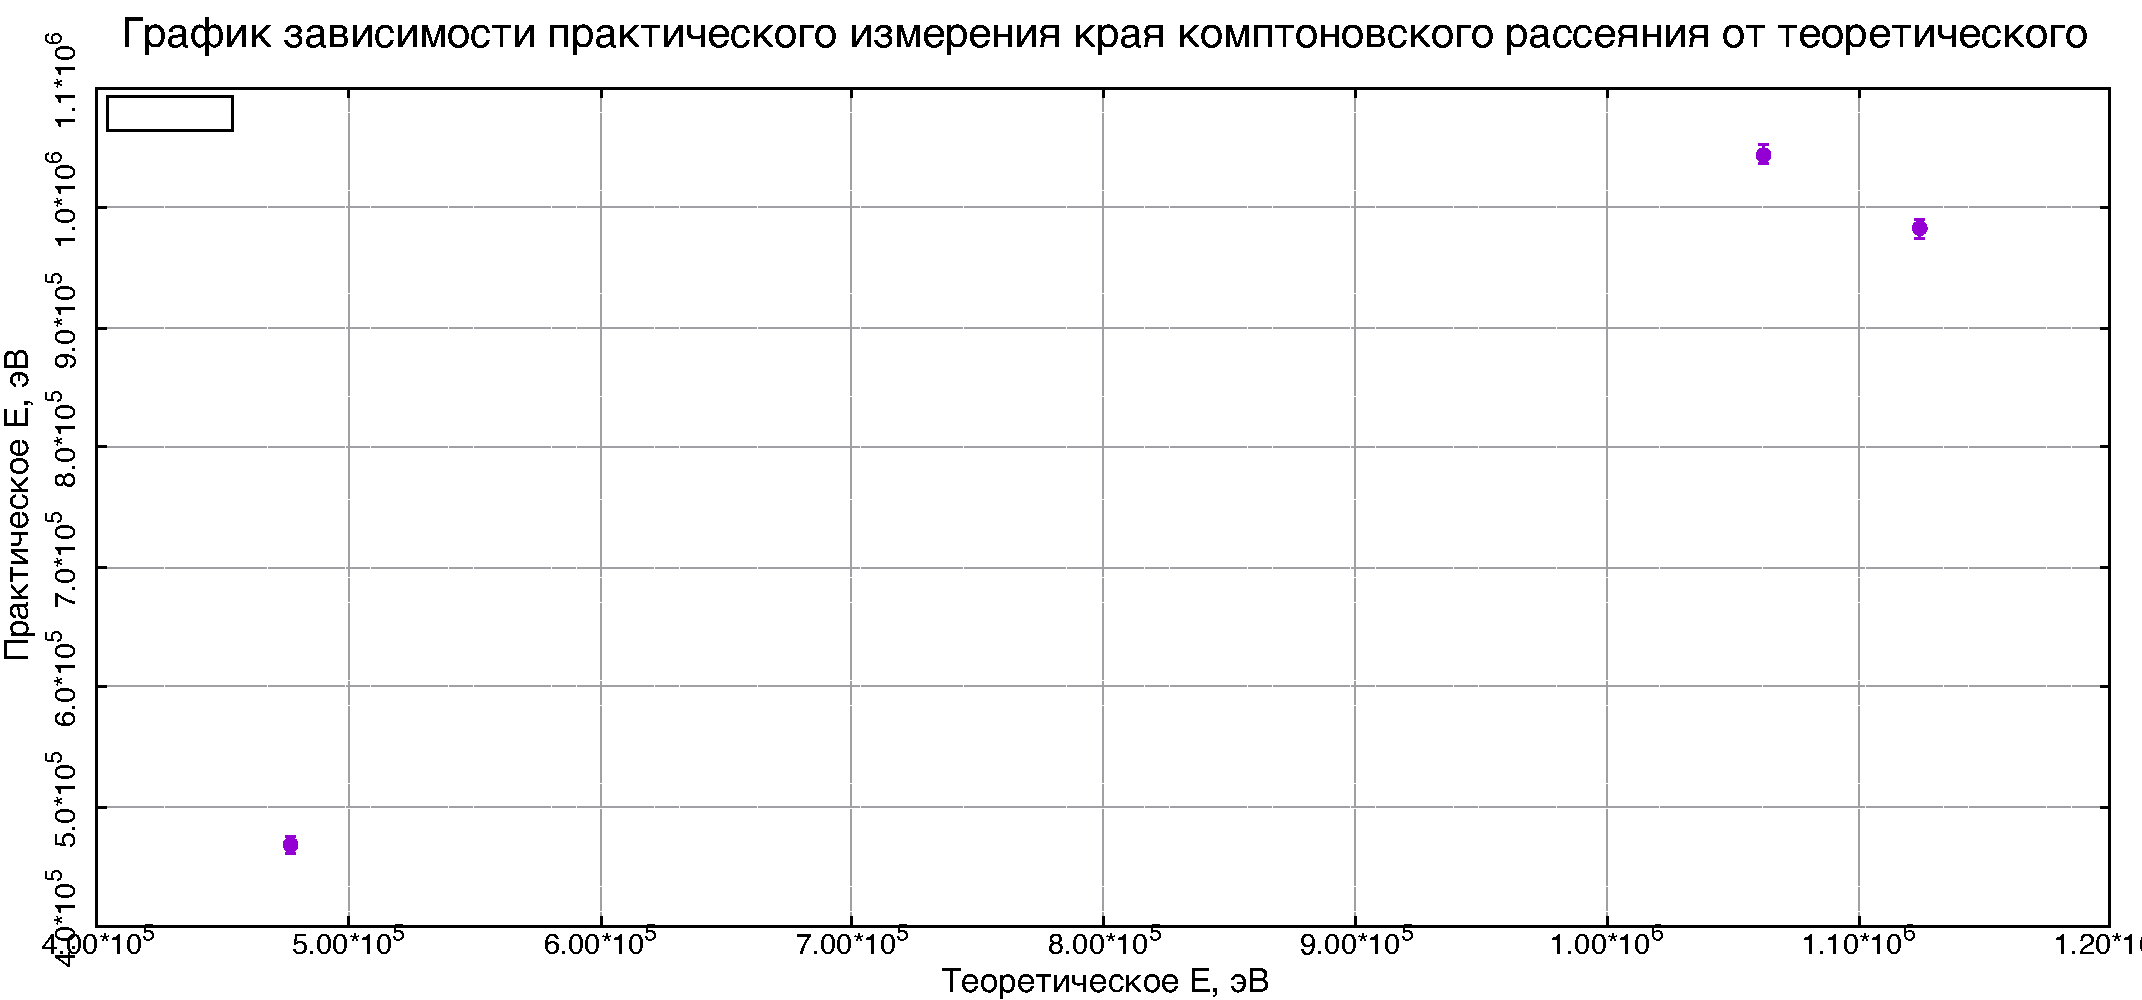
\includegraphics[width=\linewidth]{../data/compton.pdf}
	\end{figure}	


	\newpage


	\subsection{Исследование зависимости квадрата энергетического разрешения от обратной энергии пиков}
	
	\begin{figure}[h]
		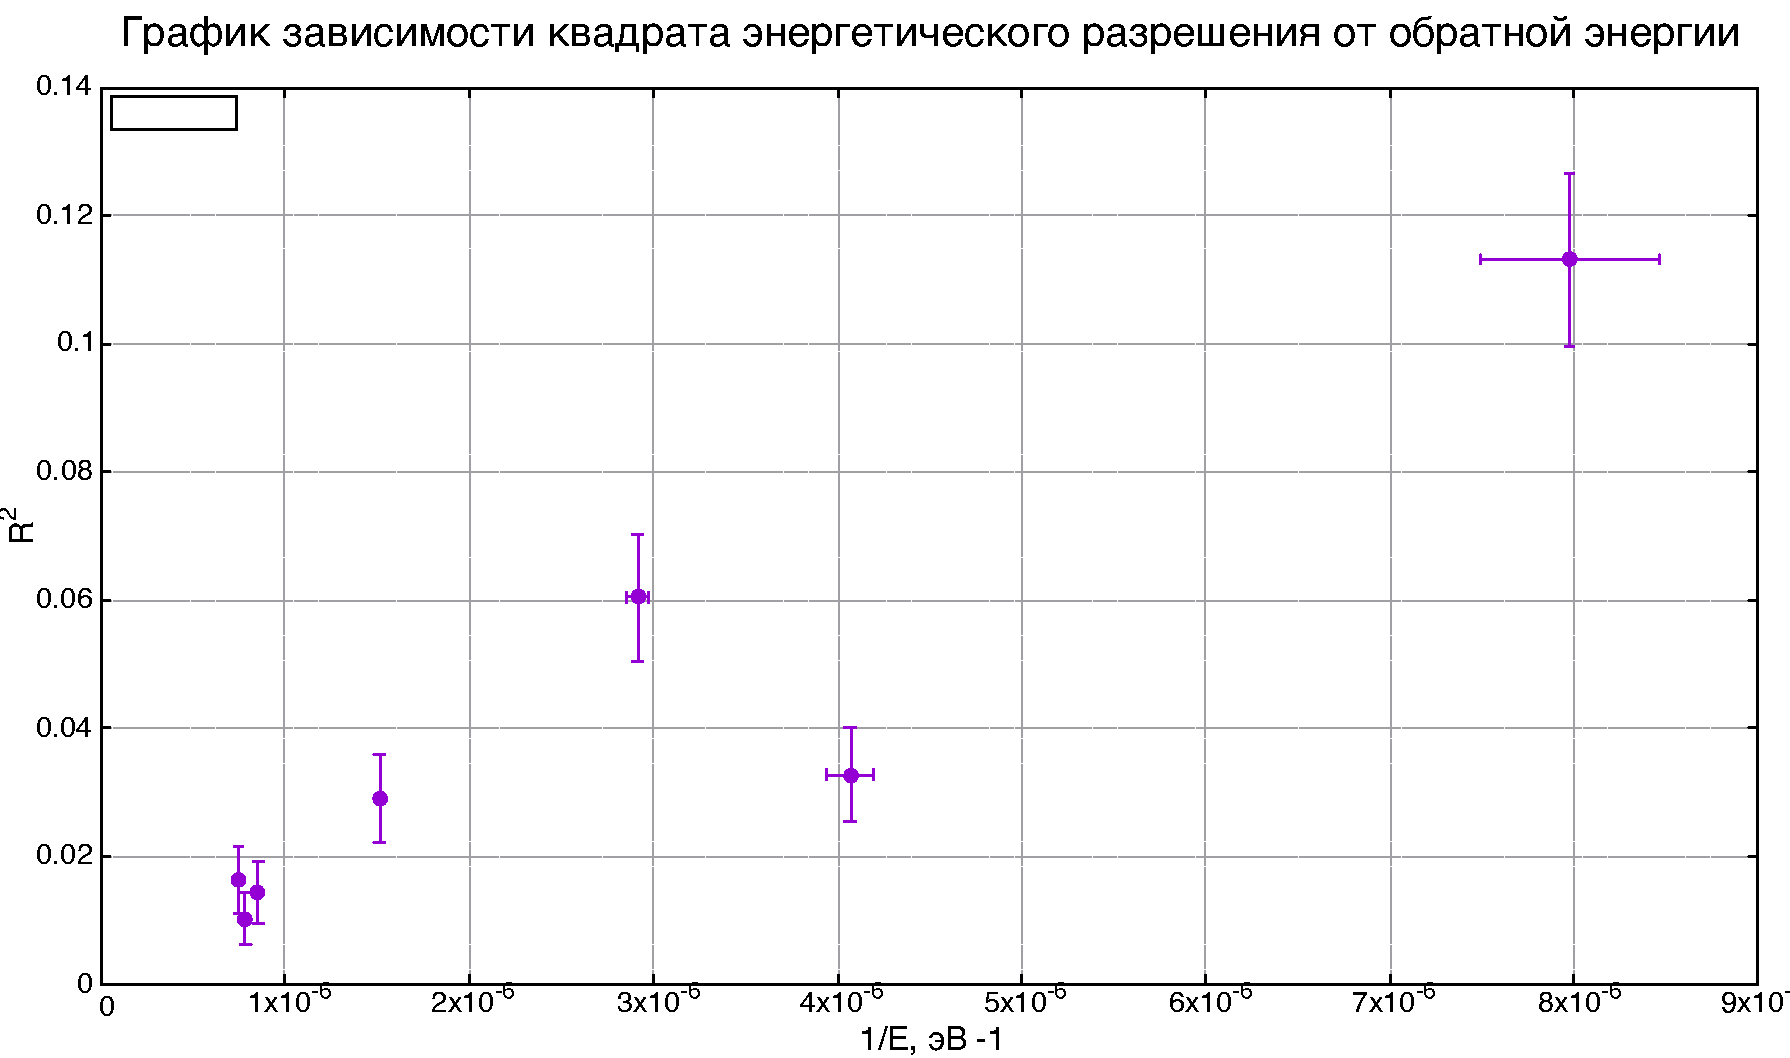
\includegraphics[width=\linewidth]{../data/re.pdf}
	\end{figure}

 	\newpage

	\subsection{Исследование пиков обратного рассеяния}
	
	Погрешность для обратного рассеяния возьмем равной погрешности измерения энергии
	
		\begin{table}[h]
		\begin{tabular}{|l|l|l|l|}
			\hline
			Элемент & Энергия. эВ   & BackScattering, эВ & \begin{tabular}[c]{@{}l@{}}Погрешность \\ измерения\\ энергии эВ\end{tabular} \\ \hline
			Co60    & 1338697.37726 & 214551.337725697   & 7669                                                                          \\ \hline
			-//-    & 1171504.45726 & 209753.646743792   & 7669                                                                          \\ \hline
			Na      & 1275041.35726 & 212848.26132574    & 7669                                                                          \\ \hline
			Cs      & 661489.35726  & 184310.242471014   & 7669                                                                          \\ \hline
			Am      & 62509.21726   & 50222.1449665474   & 7669                                                                          \\ \hline
			Eu      & 343209.25726  & 146465.023158727   & 7669                                                                          \\ \hline
			-//-    & 245807.87726  & 125280.123231252   & 7669                                                                          \\ \hline
			-//-    & 125398.29726  & 84115.0122759937   & 7669                                                                          \\ \hline
		\end{tabular}
	\end{table}
	
	\begin{figure}[h]
		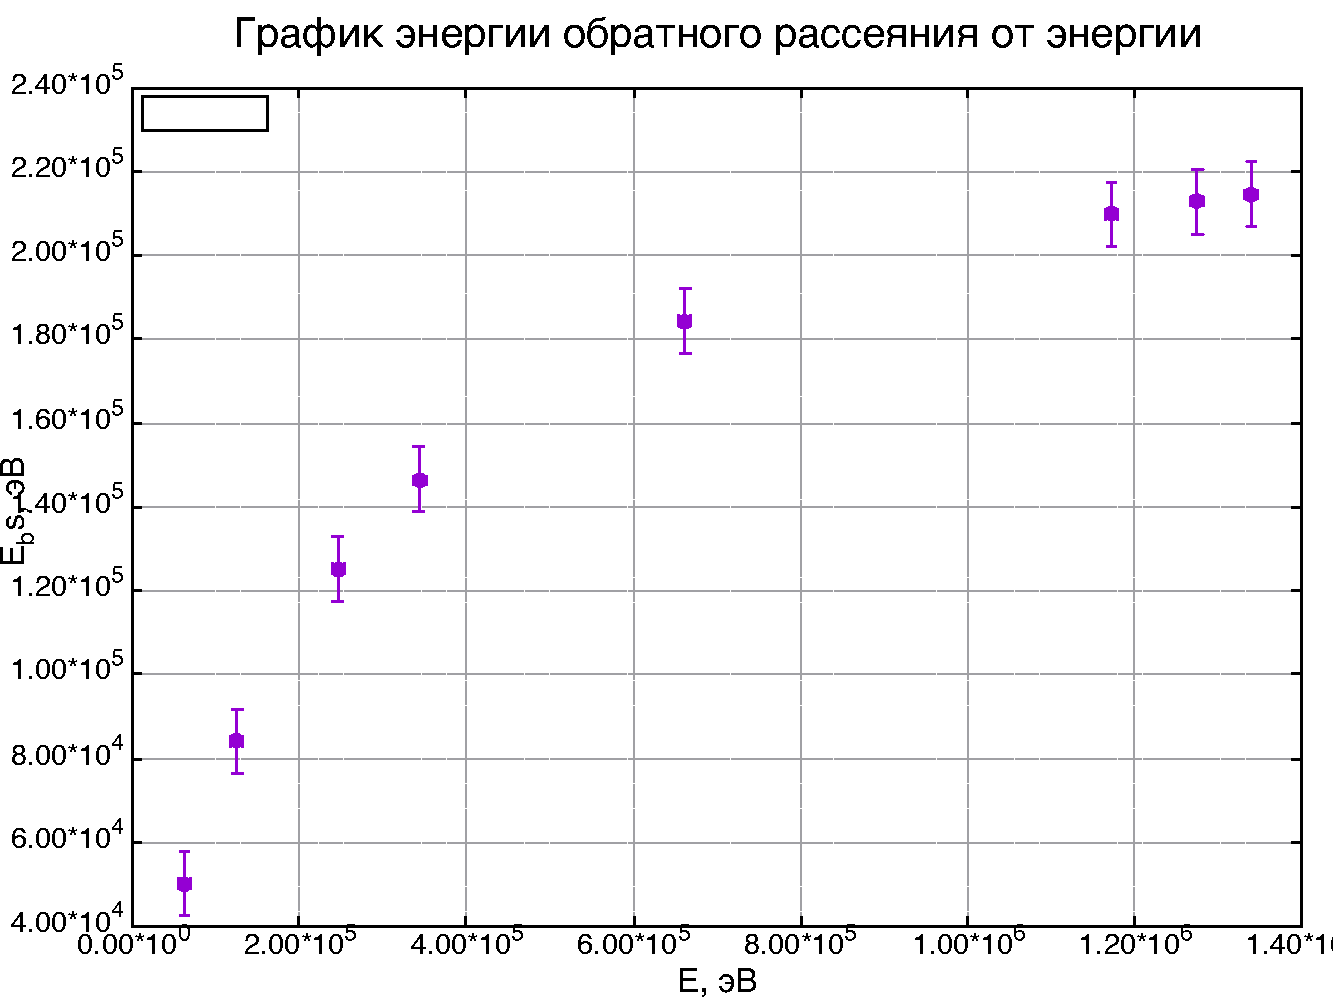
\includegraphics[width=\linewidth]{../data/bs.pdf}
	\end{figure}

	\newpage

	\subsection{Энергия наблюдаемого характеристического излучения свинца}
	
	Были измерены номера каналов пика излучения свинца длля Co60 и Na22: 
	
	\[ N_{1} = 231 \pm 10\text{ , } N_{2} = 233 \pm 10\]
	
	В пределах погрешности измерения эти пики совпадают, это говорит о том, что данный пик не зависит от типа исследуемого вещества и, следовательно, связан с постоянно присутствующим экранирующим свинцом.
	
	Энергия характеристического излучения свинца:
	
	\[E_{Pb} = 177163 \pm 7669 \text{ эВ} \]
	
	\newpage

	
	
	

\newpage
	
	
	
	

	\section{Обсуждение результатов и вывод}
	
	Я хз что тут написать я половину скатал и не понимаю сути работы

\end{document}
